% ------------------------------------------------------------------------------
% Este fichero es parte de la plantilla LaTeX para la realización de Proyectos
% Final de Grado, protegido bajo los términos de la licencia GFDL.
% Para más información, la licencia completa viene incluida en el
% fichero fdl-1.3.tex

% Copyright (C) 2012 SPI-FM. Universidad de Cádiz
% ------------------------------------------------------------------------------

Esta sección cubre el análisis del sistema de información a desarrollar, haciendo uso del lenguaje de modelado \gls{uml}.

\section{\IfLanguageName{english}{Conceptual Model}{Modelo Conceptual}}
% \question{Cuál sería mi modelo conceptual?? no tengo ``un modelo de datos''}
% A partir de los requisitos de información, se desarrollará un diagrama conceptual de clases UML, identificando las clases, atributos, relaciones, restricciones adicionales y reglas de derivación necesarias.

En la imagen \ref{image:modeloconceptual} se muestra el diagrama conceptual para \gls{kf2}.

\begin{figure}[H]
  \centering
     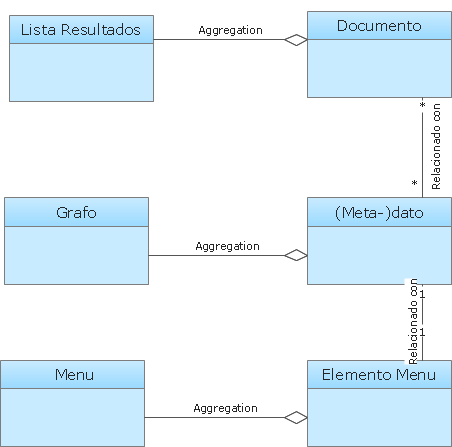
\includegraphics[width=0.7\textwidth]{Conceptual.png}
  \caption{Modelo Conceptual de \gls{kf2}}
  \label{image:modeloconceptual}
\end{figure}

\section{\IfLanguageName{english}{Use-case Model}{Modelo de Casos de Uso}}
% A partir de los requisitos funcionales descritos anteriormente, se emplearan los casos de uso como mecanismo para representar las interacciones entre los actores y el sistema bajo estudio. Para cada caso de uso deberá indicarse los actores implicados, las precondiciones y postcondiciones, los pasos que conforman el escenario principal y el conjunto de posibles escenarios alternativos.

Partiendo de los requisitos funcionales descritos en el apartado \ref{subsection:funcionales} se emplean los casos de uso para describir las interacciones de los actores y el \gls{kf2}.


\subsection{Diagramas de Casos de Uso}
En este apartado se va a describir algunos de los diagramas de caso de uso del proyecto. 

\subsection{\IfLanguageName{english}{Actors}{Actores}}
A continuación se exponen los diferentes roles que juegan los usuarios que interactúan con el sistema. Los actores pueden ser roles de personas físicas, sistemas externos o incluso el tiempo (eventos temporales).

\subsubsection{Administrador del índice de búsqueda}
Este actor será el encargado de controlar las importaciones de los datos en \gls{solr}. Puede ser una persona física que, a través de la interfaz de \gls{solr}, ejecute la importación o una tarea programada, por ejemplo un \gls{cron}.

\subsubsection{Usuario visitante}
\label{subsubsection:visitante}
Este actor utiliza la \gls{ui} sin estar registrado. No tiene autorización para iniciar sesión en el sistema. 

\subsubsection{Usuario registrado}
Este actor tiene permisos especiales concedidos por el \gls{dlr} para poder entrar en el sistema. Dependiendo de los permisos asignados, este actor dispondrá de un conjunto de documentos y campos extras. El sistema de acceso es externo al sistema.

\subsubsection{Diagrama Casos de Uso: Uso de la \gls{ui} (anónimo z registrado)}
En la imagen \ref{image:cuuiano} se representa los casos de uso para un usuario no registrado en el sistema (usuario visitante) y para uno registrado.

\begin{figure}[h!]
  \centering
     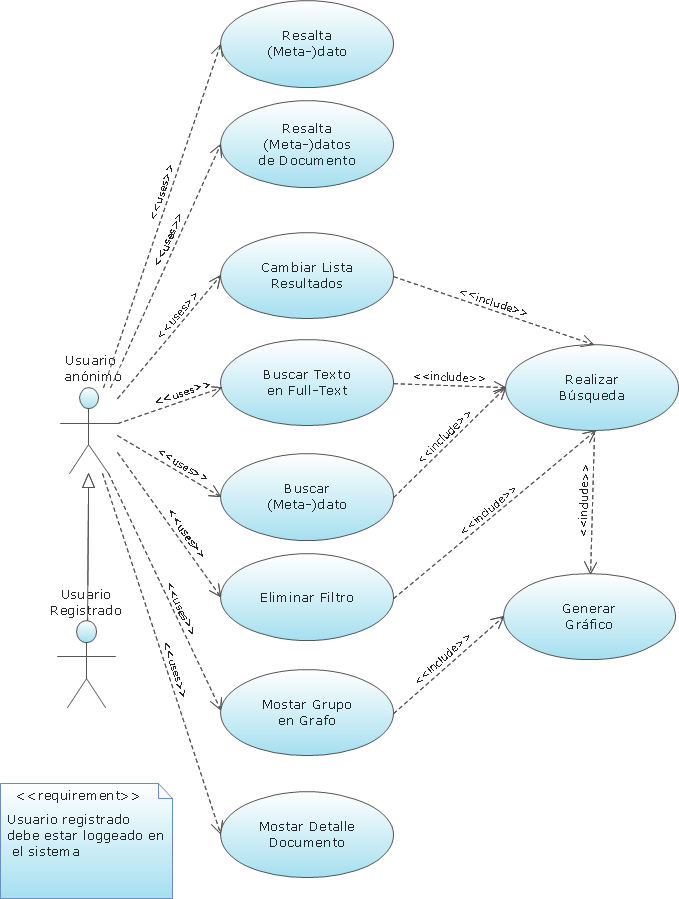
\includegraphics[width=0.8\textwidth]{UserCasesNormal.png}
  \caption{Diagrama Casos de Uso: Uso de la \gls{ui} (anónimo) y usuario registrado}
  \label{image:cuuiano}
\end{figure}

\begin{comment}
\subsubsection{Diagrama Casos de Uso: Uso de la \gls{ui}}
En la imagen \ref{image:cuuireg} se representa los casos de uso para un usuario registrado en el sistema.

\begin{figure}[h!]
  \centering
	\missingfigure{En libreta, Caso uso registrado}
  \caption{Diagrama Casos de Uso: Uso de la \gls{ui}}
  \label{image:cuuireg}
\end{figure}
\end{comment}
\subsubsection{Diagrama Casos de Uso: Gestión del índice de búsqueda}
En la imagen \ref{image:cuimport} se representa los casos de uso de un administrador del índice de búsqueda.

\begin{figure}[h!]
  \centering
     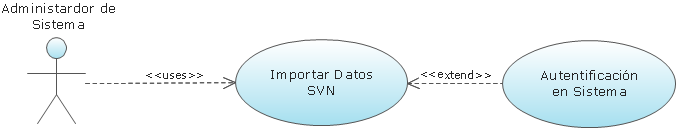
\includegraphics[width=0.8\textwidth]{UserCasesImport.png}
  \caption{Diagrama Casos de Uso: Gestión del índice de búsqueda}
  \label{image:cuimport}
\end{figure}

\subsection{Especificación de los Casos de Uso}

\subsubsection{Caso de Uso: Importación de datos}
\begin{itemize}
	\item{\textbf{Descripción}} El usuario activa la importación de los datos.
    \item{\textbf{Actor/es}} Usuario administrador del índice.
    \item{\textbf{Escenario Principal}}
    	\begin{enumerate}
        	\item El usuario selecciona una configuración a ejecutar.
			\item El usuario ejecuta importación con la configuración seleccionada.
            \item El sistema importa los documentos en el índice de búsqueda.
            \item El sistema muestra el resultado de la importación incluyendo los posibles errores.
        \end{enumerate}
\end{itemize}

\subsubsection{Caso de Uso: Buscar en \gls{fulltext}}
\begin{itemize}
	\item{\textbf{Descripción}} El usuario introduce un texto o expresión regular en el campo \gls{fulltext}.
    \item{\textbf{Actor/es}} Usuarios con o sin sesión iniciada.
    \item{\textbf{Escenario Principal}}
    	\begin{enumerate}
        	\item Usuario entra el texto a buscar en el campo \gls{fulltext}.
        	\item El sistema actualiza la lista de documentos únicamente con los elementos que contienen el texto introducido.
            \item El sistema actualiza el grafo de visualización con los nuevos valores de los \glspl{metadato} de los documentos encontrados (actualiza el tamaño de los nodos y de las relaciones entre ellos).
            \item El sistema actualiza los valores de los contadores en el menú.
            \item El sistema añade el valor introducido a la lista de filtros activos.
            \item El sistema sitúa la paginación en su primera página.
        \end{enumerate}
%    \sitem{Escenario Alternativo}
\end{itemize}



\subsubsection{Caso de Uso: Buscar \gls{metadato}}
\begin{itemize}
	\item{\textbf{Descripción}} El usuario filtra los documentos por un \gls{metadato} a través del grafo de visualización o del menú.
    \item{\textbf{Actor/es}} Usuarios con o sin sesión iniciada.
    \item{\textbf{Escenario Principal}}
    	\begin{enumerate}
        	\item Usuario pulsa sobre un nodo el nodo del grafo o sobre el elemento de la tabla que desea filtrar.
        	\item El sistema actualiza la lista de documentos suprimiendo aquellos que no contienen \gls{metadato} seleccionado.
            \item El sistema actualiza el grafo de visualización con los nuevos valores de los \glspl{metadato} de los documentos encontrados (actualiza el tamaño de los nodos y de las relaciones entre ellos).
            \item El sistema actualiza los valores de los contadores en el menú.
            \item El sistema añade el \gls{metadato} a la lista de filtros activos.
            \item El sistema sitúa la paginación en su primera página. 
        \end{enumerate}
    \item{\textbf{Escenario Alternativo}}
    	\begin{enumerate}[label=2.\alph*]
    		\item El \gls{metadato} seleccionado se muestra en el grafo.
            \begin{enumerate}[label=\arabic*]
            	\item El sistema elimina el elemento del grafo..
            	\item Continuar con el paso 3.
            \end{enumerate}
        \end{enumerate}
\end{itemize}

\subsubsection{Caso de Uso: Detalles de documento}
\begin{itemize}
	\item{\textbf{Descripción}} El usuario de \gls{ui} obtiene los detalles de un documento en una ventana emergente.
    \item{\textbf{Actor/es}} Usuarios con o sin sesión iniciada.
    \item{\textbf{Escenario Principal}}
    	\begin{enumerate}
        	\item Usuario selecciona un elemento de la lista de resultados.
        	\item El sistema despliega el acordeón del elemento.
            \item El usuario pulsa el botón para ver los detalles del documento.
            \item El sistema abre una ventana emergente donde muestra los campos permitidos para el usuario.
        \end{enumerate}
\end{itemize}

\subsubsection{Caso de Uso: Eliminar filtro}
\begin{itemize}
	\item{\textbf{Descripción}} El usuario de \gls{ui} elimina un filtro de los actuales activos en la lista filtros activos.
    \item{\textbf{Actor/es}} Usuarios con o sin sesión iniciada.
    \item{\textbf{Escenario Principal}}
    	\begin{enumerate}
        	\item Usuario selecciona un elemento de la lista formada por los filtros que con anterioridad fueron activados.
			\item El sistema actualiza la lista de documentos aplicando el resto de filtros que todavía siguen activos.
            \item El sistema actualiza el grafo de visualización con los nuevos valores de los \glspl{metadato} de los documentos encontrados (actualiza el tamaño de los nodos y de las relaciones entre ellos).
            \item El sistema actualiza los valores de los contadores en el menú.
            \item El sistema suprime el filtro la lista de filtros activos.
            \item El sistema sitúa la paginación en su primera página.
        \end{enumerate}
\end{itemize}


\subsubsection{Caso de Uso: Cambiar lista de resultados}
\begin{itemize}
	\item{\textbf{Descripción}} El usuario de \gls{ui} modifica la lista de los resultados cambiando la paginación o el criterio de ordenación.
    \item{\textbf{Actor/es}} Usuarios con o sin sesión iniciada.
    \item{\textbf{Escenario Principal}}
    	\begin{enumerate}
        	\item Usuario selecciona una página de la lista de paginación.
			\item El sistema actualiza la lista de documentos mostrando únicamente los elementos de esa página.
        \end{enumerate}
    \item{\textbf{Escenario Alternativo}}
    	\begin{enumerate}[label=2.\alph*]
    		\item El usuario selecciona otro criterio de ordenación para la lista de resultados.
            \begin{enumerate}[label=\arabic*]
            	\item El sistema actualiza la lista de documentos mostrándolos en el orden seleccionado, sin cambiar la página donde se encontraba anteriormente.
            \end{enumerate}
        \end{enumerate}
\end{itemize}


\subsubsection{Caso de Uso: Resaltar \gls{metadato}}
\begin{itemize}
	\item{\textbf{Descripción}} El usuario de \gls{ui} resalta las relaciones de un \gls{metadato}.
    \item{\textbf{Actor/es}} Usuarios con o sin sesión iniciada.
    \item{\textbf{Escenario Principal}}
    	\begin{enumerate}
        	\item Usuario se sitúa sobre un \gls{metadato} en el grafo o en el menú.
			\item El sistema muestra menos nítido los elementos del grafo que no tienen relación con este \gls{metadato}.
            \item El sistema muestra resaltado los documentos de la actual página de resultados que contienen este \gls{metadato}.
            \item El sistema muestra una pequeña ventana con información adicional sobre este \gls{metadato}.
        \end{enumerate}
    \item{\textbf{Escenario Alternativo}}
    	\begin{enumerate}[label=2.\alph*]
    		\item El \gls{metadato} seleccionado tiene subelementos en el menú.
            \begin{enumerate}[label=\arabic*]
            	\item El sistema muestra menos nítido los elementos del grafo que no tienen relación con ningún subelemento.
                \item El sistema muestra resaltado los documentos de la actual página de resultados que contienen algún subelemento. 
            \end{enumerate}
        \end{enumerate}
\end{itemize}


\subsubsection{Caso de Uso: Resaltar \glspl{metadato} de documento}
\begin{itemize}
	\item{\textbf{Descripción}} El usuario de \gls{ui} resalta las relaciones de un documento.
    \item{\textbf{Actor/es}} Usuarios con o sin sesión iniciada.
    \item{\textbf{Escenario Principal}}
    	\begin{enumerate}
        	\item Usuario se sitúa sobre un documento de la lista de resultados.
			\item El sistema muestra menos nítido los elementos del grafo que no tienen relación con este documento.
            \item El sistema muestra resaltado en el menú los elementos los \glspl{metadato} del documento.
        \end{enumerate}
\end{itemize}


\subsubsection{Caso de Uso: Mostrar grupo en grafo}
\begin{itemize}
	\item{\textbf{Descripción}} El usuario de \gls{ui} selecciona un grupo para mostrar en el grafo.
    \item{\textbf{Actor/es}} Usuarios con o sin sesión iniciada.
    \item{\textbf{Escenario Principal}}
    	\begin{enumerate}
        	\item Usuario selecciona un grupo del menú.
			\item El sistema añade los subelementos del grupo en el grafo.
        \end{enumerate}
    \item{\textbf{Escenario Alternativo}}
    	\begin{enumerate}[label=2.\alph*]
    		\item El grupo seleccionado ya se está mostrando en el menú.
            \begin{enumerate}[label=\arabic*]
			\item El sistema elimina del grafo los subelementos del grupo.
            \end{enumerate}
        \end{enumerate}
\end{itemize}


\section{\IfLanguageName{english}{Behavioral model}{Modelo de Comportamiento}}
\begin{comment}[inline]{
A partir de los casos de uso anteriores, se crea el modelo de comportamiento. Para ello, se realizarán los diagramas de secuencia del sistema, donde se identificarán las operaciones o servicios del sistema. Luego, se detallará el contrato de las operaciones identificadas.
}
\end{comment}
Partiendo de los casos de uso anteriores, se detallan ahora los modelos de comportamiento asociados.\\

\subsubsection{Caso de Uso: Importación de datos}
\begin{figure}[H]
  \centering
     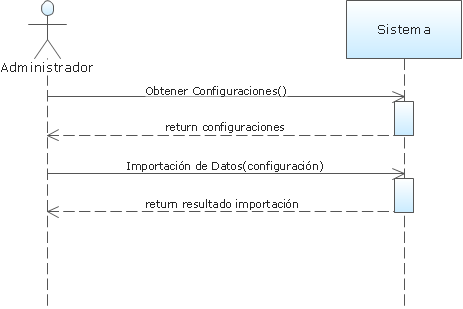
\includegraphics[width=0.7\textwidth]{DCImportacion.png}
  \caption{Modelo de Comportamiento Caso de Uso: Importación de datos}
  \label{image:compoimport}
\end{figure}
\subsubsection{Caso de Uso: Buscar en \gls{fulltext}}
\begin{figure}[H]
  \centering
     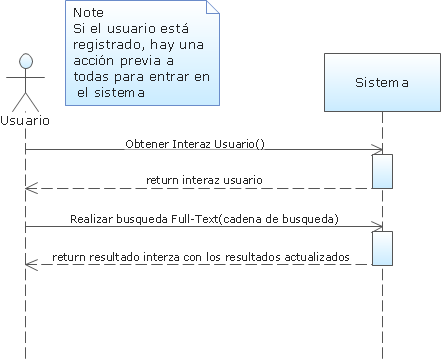
\includegraphics[width=0.7\textwidth]{DCfulltext.png}
  \caption{Modelo de Comportamiento aso de Uso: Buscar en \gls{fulltext}}
  \label{image:compofulltext}
\end{figure}
\subsubsection{Caso de Uso: Buscar \gls{metadato}}
\begin{figure}[H]
  \centering
     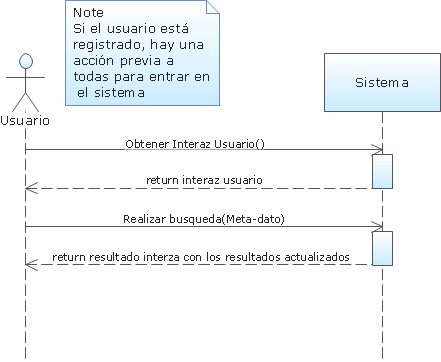
\includegraphics[width=0.7\textwidth]{DCmetadato.png}
  \caption{Modelo de Comportamiento Caso de Uso: Buscar \gls{metadato}}
  \label{image:compobusmeta}
\end{figure}
\subsubsection{Caso de Uso: Detalles de documento}
\begin{figure}[H]
  \centering
     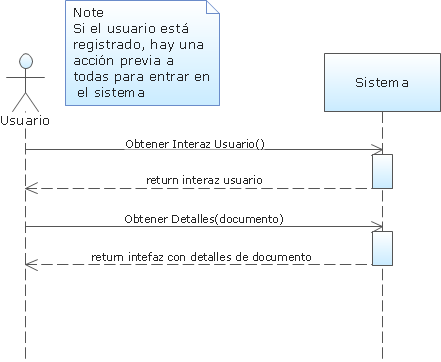
\includegraphics[width=0.7\textwidth]{DCDetalles.png}
  \caption{Modelo de Comportamiento Caso de Uso: Detalles de documento}
  \label{image:compodetalles}
\end{figure}
\subsubsection{Caso de Uso: Eliminar filtro}
\begin{figure}[H]
  \centering
     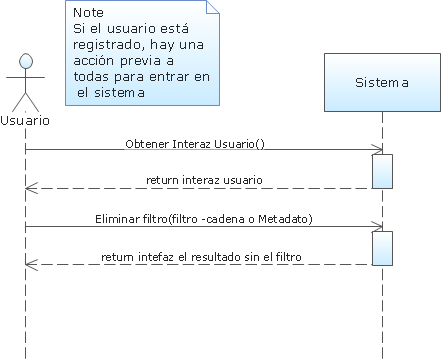
\includegraphics[width=0.7\textwidth]{DCeliminar.png}
  \caption{Modelo de Comportamiento Caso de Uso: Eliminar filtro}
  \label{image:compoelimina}
\end{figure}
\subsubsection{Caso de Uso: Cambiar lista de resultados}
\begin{figure}[H]
  \centering
     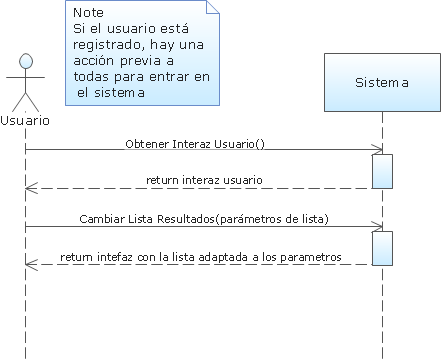
\includegraphics[width=0.7\textwidth]{DCcambialista.png}
  \caption{Modelo de Comportamiento Caso de Uso: Cambiar lista de resultados}
  \label{image:compocambia}
\end{figure}
\subsubsection{Caso de Uso: Resaltar \gls{metadato}}
\begin{figure}[H]
  \centering
     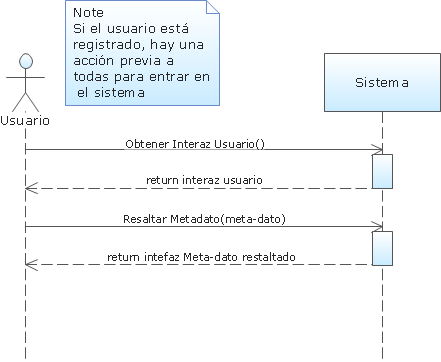
\includegraphics[width=0.7\textwidth]{DCresaltaMetadato.png}
  \caption{Modelo de Comportamiento Caso de Uso: Resaltar \gls{metadato}}
  \label{image:compresalmeta}
\end{figure}
\subsubsection{Caso de Uso: Resaltar \glspl{metadato} de documento}
\begin{figure}[H]
  \centering
     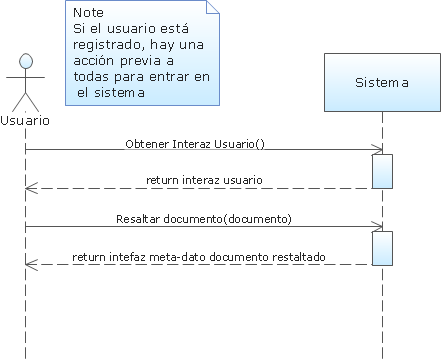
\includegraphics[width=0.7\textwidth]{DCresaltaDocu.png}
  \caption{Modelo de Comportamiento Caso de Uso: Resaltar \glspl{metadato} de documento}
  \label{image:comporesaldoc}
\end{figure}
\subsubsection{Caso de Uso: Mostrar grupo en grafo}
\begin{figure}[H]
  \centering
     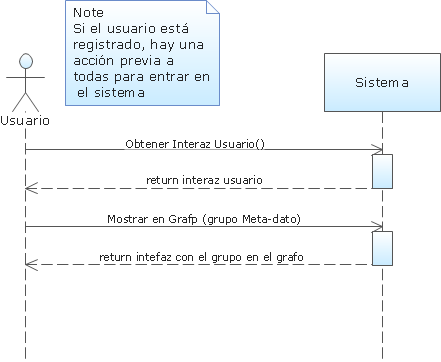
\includegraphics[width=0.7\textwidth]{DCmostrarGrupo.png}
  \caption{Modelo de Comportamiento Caso de Uso: Mostrar grupo en grafo}
  \label{image:compogropopgrafo}
\end{figure}


\section{\IfLanguageName{english}{User-interface Model}{Modelo de Interfaz de Usuario}} 
%En esta sección se deberá incluir un prototipo de baja fidelidad o mockup de la interfaz de usuario del sistema. Además, es preciso elaborar un diagrama de navegación, reflejando la secuencia de pantallas a las que tienen acceso los diferentes roles de usuario y la conexión entre éstas.

A continuación mostramos unos prototipos de baja fidelidad de la interfaz de usuario. En la imagen \ref{image:mockup1} podemos ver la estructura de la pantalla general de la aplicación.\\

\begin{figure}[h!]
  \centering
     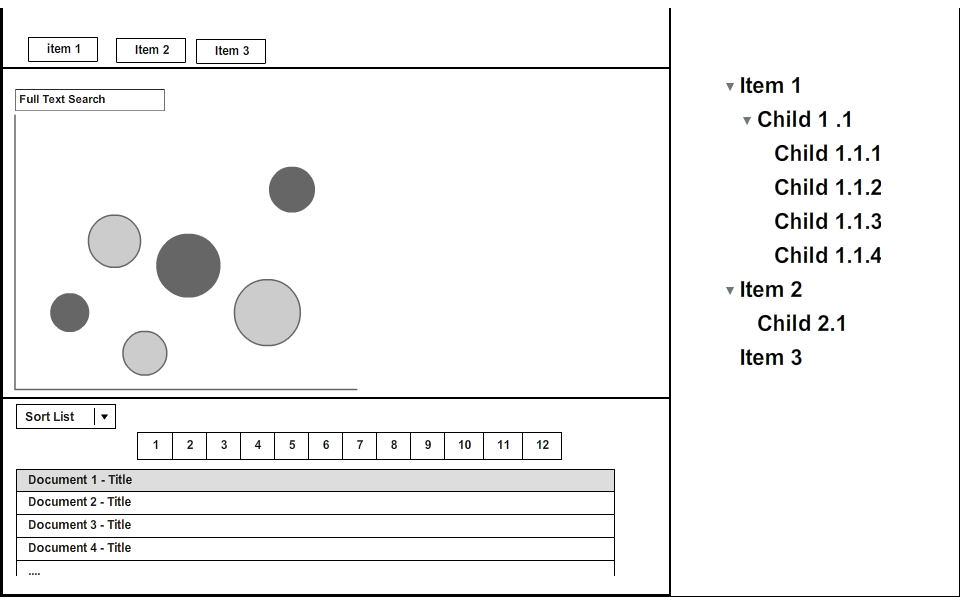
\includegraphics[width=0.8\textwidth]{mock1.png}
  \caption{Mockup - pantalla general \gls{kf2}}
  \label{image:mockup1}
\end{figure}

Cuando en usuario visualiza los detalles de un documento la pantalla tiene una semejanza a la expuesta en la imagen \ref{image:mockup2}.

\begin{figure}[h!]
  \centering
     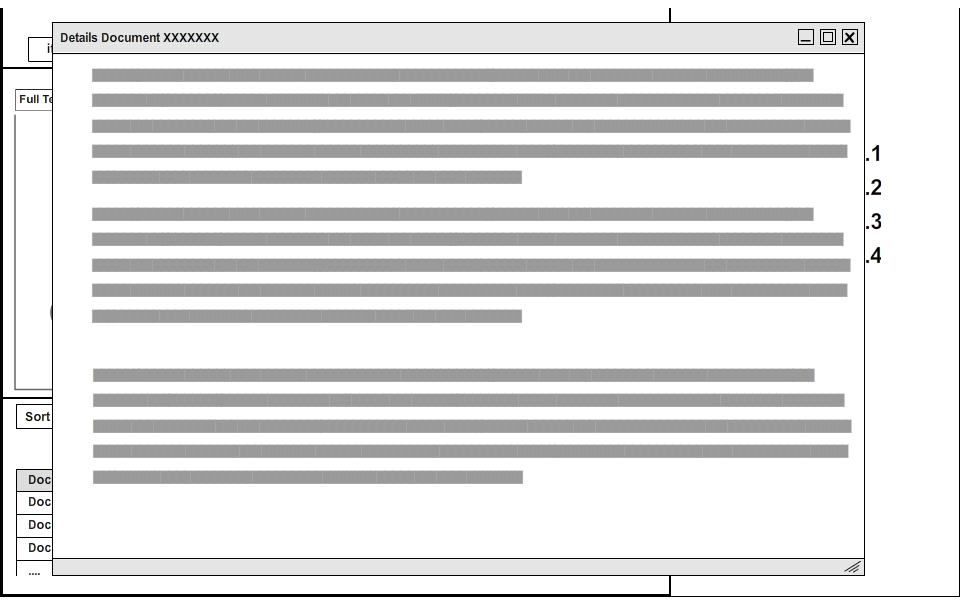
\includegraphics[width=0.8\textwidth]{mock2.png}
  \caption{Mockup - pantalla de detalles en \gls{kf2}}
  \label{image:mockup2}
\end{figure}
